
%\documentstyle[epsf,twocolumn]{jarticle}       %LaTeX2e仕様
\documentclass[twocolumn]{jarticle}     %pLaTeX2e仕様(platex.exeの場合)
% \documentclass[onecolumn]{ujarticle}   %pLaTeX2e仕様(uplatex.exeの場合)
%%%%%%%%%%%%%%%%%%%%%%%%%%%%%%%%%%%%%%%%%%%%%%%%%%%%%%%%%%%%%%
%%
%%  基本バージョン
%%
%%%%%%%%%%%%%%%%%%%%%%%%%%%%%%%%%%%%%%%%%%%%%%%%%%%%%%%%%%%%%%%%
\setlength{\topmargin}{-45pt}
%\setlength{\oddsidemargin}{0cm}
\setlength{\oddsidemargin}{-7.5mm}
%\setlength{\evensidemargin}{0cm}
\setlength{\textheight}{24.1cm}
%setlength{\textheight}{25cm}
\setlength{\textwidth}{17.4cm}
%\setlength{\textwidth}{172mm}
\setlength{\columnsep}{11mm}

%\kanjiskip=.07zw plus.5pt minus.5pt


% 【節が変わるごとに (1.1)(1.2) … (2.1)(2.2) と数式番号をつけるとき】
%\makeatletter
%\renewcommand{\theequation}{%
%\thesection.\arabic{equation}} %\@addtoreset{equation}{section}
%\makeatother

%\renewcommand{\arraystretch}{0.95} 行間の設定
%%%%%%%%%%%%%%%%%%%%%%%%%%%%%%%%%%%%%%%%%%%%%%%%%%%%%%%%
%\usepackage{graphicx}   %pLaTeX2e仕様(\documentstyle ->\documentclass)
\usepackage[dvipdfmx]{graphicx}
\usepackage{subcaption}
\usepackage{multirow}
\usepackage{amsmath}
\usepackage{url}
\usepackage{ulem}
\usepackage{algorithm}
\usepackage{algorithmic}
\usepackage{listings} %,jlisting} %日本語のコメントアウトをする場合jlistingが必要
%ここからソースコードの表示に関する設定
\lstset{
  basicstyle={\ttfamily},
  identifierstyle={\small},
  commentstyle={\smallitshape},
  keywordstyle={\small\bfseries},
  ndkeywordstyle={\small},
  stringstyle={\small\ttfamily},
  frame={tb},
  breaklines=true,
  columns=[l]{fullflexible},
  numbers=left,
  xrightmargin=0zw,
  xleftmargin=3zw,
  numberstyle={\scriptsize},
  stepnumber=1,
  numbersep=1zw,
  lineskip=-0.5ex
}
\newcommand{\argmax}{\mathop{\rm arg~max}\limits}
\newcommand{\argmin}{\mathop{\rm arg~min}\limits}

%%%%%%%%%%%%%%%%%%%%%%%%%%%%%%%%%%%%%%%%%%%%%%%%%%%%%%%%
\begin{document}

	%bibtex用の設定
	%\bibliographystyle{ujarticle}

	\twocolumn[
		\noindent
		\hspace{1em}
		2021 年 6 月 18 日
		ゼミ資料
		\hfill
		M1 杉山 竜弥
		\vspace{2mm}

		\hrule
		\begin{center}
			{\Large \bf 進捗報告}
		\end{center}
		\hrule
		\vspace{9mm}
	]


\section{今週やったこと}
\begin{itemize}
  \item 対話タスクの動作確認
\end{itemize}

\section{英語での対話}

\begin{figure}[tb]
  \begin{center}
    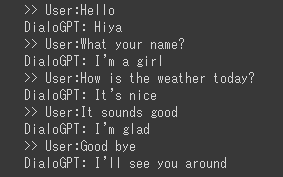
\includegraphics[clip,width=75mm]{ss.png}
    \caption{対話例}
    \label{fig:con}
  \end{center}
\end{figure}

図 \ref{fig:con} に対話例を示した.
英語の場合, 対話を自然に続けられることを確認した.



\section{日本語での対話}

Tokenizer がテキストを前処理し, Model が出力するという関係になっている.
Tokenizer にエラーが起きて, 動かすことができなかった.

GPTに準拠するならBPE(Byte Pair Encoding)によって単語を分解し Token に置き換えるが,
日本語には文字の種類が多いことや空白がないことなどが原因で適切な Tokenizer を英語のものとは変える必要がある.
BPEの他に, 形態素解析 (Mecab) を元にした BERT の Tokenizer もある.
学習の前提となるので, 学習済みパラメータがどのような Tokenizer を使用したのかを見なければならないが, github の README を見ても情報が少なく現在は動作を確認する段階に至れなかった.


% \begin{table}[tb]
%   \begin{center}
%     \caption{GPT-2の解けるタスク}
%     \begin{tabular}{|c|} \hline
%       % AutomaticSpeechRecognition \\ \hline
%       Conversational \\ \hline
%       % FeatureExtraction \\ \hline
%       % FillMask \\ \hline
%       % ImageClassification \\ \hline
%       QuestionAnswering \\ \hline
%       Summarization \\ \hline
%       TextClassification \\ \hline
%       TextGeneration \\ \hline
%       % TokenClassification \\ \hline
%       Translation \\ \hline
%       % ZeroShotClassification \\ \hline
%       % Text2TextGeneration \\ \hline
%       % TableQuestionAnswering \\ \hline
%     \end{tabular}
%     \label{tab:task}
%   \end{center}
% \end{table}
% \url{https://huggingface.co/}

\section{今後の予定}
% なんとなくなんかの勉強をするとかではなく具体的に
\begin{itemize}
  \item 日本語での対話タスクの動作確認
\end{itemize}

% 参考文献リスト
\bibliographystyle{unsrt}
\bibliography{ref}
\end{document}
